The transport of a scalar according to a parabolic function and 
submitted to a monophase flow of a Newtonian and incompressible fluid 
with a high number of \textit{Reynolds} 
($\textit{Re} \rightarrow \infty$) is known as a 
\textit{Pure Advection flow}. In this type of flow, 
it is expected that the scalar will not diffuse. 
For approximation methods like \textit{FEM} and \textit{FDM}, 
it is possible to observe the presence of spurious oscillations. 
As mentioned earlier, several schemes can be used to reduce these 
numerical oscillations. In this section, we will present the use 
of the \textit{semi-Lagrangian} scheme to reduce spurious oscillations 
compared to the \textit{Taylor-Galerkin} Method. 
The \ref{conveccao} presents schematically the problem and 
the dynamics of scalar transport.

\vspace{0.5cm}
\begin{figure}[H]
\begin{center}
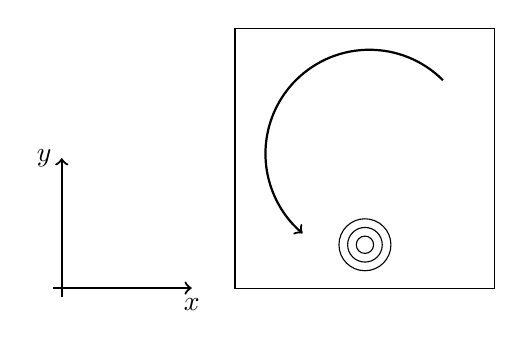
\begin{tikzpicture}[scale=1.1]
 \draw (0,0) -- (3,0) -- (3,3) -- (0,3) -- cycle;

 \draw [->,thick] (2.4,2.4) arc (45:230:1.2);
 
 \draw [->,thick] (-2,-0.1)--(-2,1.5) node[left] {$y$};
 \draw [->,thick] (-2.1,0)--(-0.5,0) node[below] {$x$};

 \draw (1.5,0.5) circle (0.3);
 \draw (1.5,0.5) circle (0.2);
 \draw (1.5,0.5) circle (0.1);

\end{tikzpicture}
\end{center}
\caption{Transport of a scalar in Pure Advection Flow.}
\label{conveccao}
\end{figure}

\medskip
\noindent
The scalar transport $\alpha$ for a pure advection flow is shown below:


\begin{equation}
 \frac{\partial \alpha}{\partial t} 
 + 
 \textbf{c} \cdot \nabla \alpha
 = 0
\end{equation}

\noindent
where is relative velocity and it is calculated by 
$\textbf{c} = \textbf{v} - \hat{\textbf{v}}$,
$\textbf{v}$ is material velocity field and its components are
defined as: $u = -y$ e $v = x$,
$\hat{\textbf{v}}$ is the mesh velocity and it is calculated
by the Eq. \ref{mesh velocity eq}. 
Therefore, it is expected that given an initial scalar field, 
it will be displaced by the velocity field without diffusion, 
that is, its profile should not be changed while the flow occurs. 
Any change in the scalar field profile is considered a numerical error.
The initial scalar field was defined by a parabolic
profile $c = 1 - x^2 - y^2$, where $x$ and $y$ are the spatial components.



\medskip
The \ref{perfil c} presents the comparison between the scalar field
profile $c$ for the semi-Lagrangian and Taylor-Galerkin methods in 
several positions on the axis of rotation as the flow occurs. 
It is possible to observe that in both methods the spurious oscillations 
are presented. In the Taylor-Galerkin method, however, 
such oscillations are dampened in contrast to the Galerkin method 
where we can observe that spurious oscillations increase and 
the scalar field profile becomes completely distorted.

\begin{center}
\begin{figure}[H]
     \centering
     \begin{minipage}{.5\linewidth}
      \centering
      \includegraphics[scale=0.53]{./02_chaps/cap_validation/figure/convection_0.pdf}\\
      (a)
     \end{minipage}%
     \begin{minipage}{.5\linewidth}
      \centering
      \includegraphics[scale=0.53]{./02_chaps/cap_validation/figure/convection_300.pdf}\\
      (b)
     \end{minipage}
     \begin{minipage}{.5\linewidth}
      \centering
      \includegraphics[scale=0.53]{./02_chaps/cap_validation/figure/convection_600.pdf}\\
      (c)
     \end{minipage}%
     \begin{minipage}{.5\linewidth}
      \centering
      \includegraphics[scale=0.53]{./02_chaps/cap_validation/figure/convection_950.pdf}\\
      (d)
     \end{minipage}
     \medskip
     \caption{Comparison of $c$ profile for the Galerkin e Taylor-Galerkinmethod in several positions on the axis of rotation: 
     (a) initial, 
     (b) 1/4 rotation,
     (c) 1/2 rotation and
     (d) 3/4 rotation.}
     \label{perfil c}
\end{figure}
\end{center}

\vspace{-1cm}
The \ref{galerkin} and \ref{taylor} show the spatial arrangement 
of spurious oscillations for the Galerkin and Taylor-Galerkin methods 
respectively. As mentioned earlier, the oscillations presented 
in the Galerkin method completely distort the scalar field $c$ 
while in the Taylor-Galerkin method, they are dampened as expected. 
Therefore, for problems where spurious oscillations are present, 
the Taylor-Galerkin method is superior to the Galerkin method.

\vspace{0.5cm}
\begin{figure}[H]
     \centering
     \begin{minipage}{.5\linewidth}
      \centering
      \includegraphics[scale=0.2]{./02_chaps/cap_validation/figure/galerkin_0.png}\\
      (a)
     \end{minipage}%
     \begin{minipage}{.5\linewidth}
      \centering
      \includegraphics[scale=0.2]{./02_chaps/cap_validation/figure/galerkin_300.png}\\
      (b)
     \end{minipage}
     \begin{minipage}{.5\linewidth}
      \centering
      \includegraphics[scale=0.2]{./02_chaps/cap_validation/figure/galerkin_600.png}\\
      (c)
     \end{minipage}%
     \begin{minipage}{.5\linewidth}
      \centering
      \includegraphics[scale=0.21]{./02_chaps/cap_validation/figure/galerkin_950.png}\\
      (d)
     \end{minipage}
     \medskip
     \caption{
Spurious oscillations for the Galerkin method in several positions of the axis of rotation:	
     (a) initial, 
     (b) 1/4 rotation,
     (c) 1/2 rotation and
     (d) 3/4 rotation.}
     \label{galerkin}
\end{figure}

\begin{figure}[H]
     \centering
     \begin{minipage}{.5\linewidth}
      \centering
      \includegraphics[scale=0.2]{./02_chaps/cap_validation/figure/taylor_0.png}\\
      (a)
     \end{minipage}%
     \begin{minipage}{.5\linewidth}
      \centering
      \includegraphics[scale=0.2]{./02_chaps/cap_validation/figure/taylor_300.png}\\
      (b)
     \end{minipage}
     \begin{minipage}{.5\linewidth}
      \centering
      \includegraphics[scale=0.2]{./02_chaps/cap_validation/figure/taylor_600.png}\\
      (c)
     \end{minipage}%
     \begin{minipage}{.5\linewidth}
      \centering
      \includegraphics[scale=0.2]{./02_chaps/cap_validation/figure/taylor_950.png}\\
      (d)
     \end{minipage}
     \medskip
     \caption{
Spurious oscillations for the Taylor-Galerkin method in several positions of the axis of rotation:	
     (a) initial, 
     (b) 1/4 rotation,
     (c) 1/2 rotation and
     (d) 3/4 rotation.}
     \label{taylor}
\end{figure}

